\documentclass[usenames,dvipsnames]{beamer}
\usetheme{Boadilla}
\usepackage{hyperref}
\usepackage{graphicx}
\usepackage{multimedia}
% mwe needs to be installed for the example images to show
%\usepackage{mwe}
\usepackage{fontawesome}
\usepackage{fancyvrb}
\usepackage{soul}
\usepackage{multicol}
\usepackage{optparams}
\usepackage{adjustbox}
\usepackage{tikz}
\usetikzlibrary{shapes,positioning}
\usepackage{subfig}
\usepackage[
    backend=biber,
    natbib=true,
    sorting=none,
    style=verbose-ibid,
    mincitenames=2,
    maxcitenames=2,
    citestyle=authoryear,
]{biblatex}
\addbibresource{citations.bib}
\usepackage{pgfpages}
\usepackage{xcolor}
\usepackage{minted}
\definecolor{ao(english)}{rgb}{0.0, 0.5, 0.0}
\definecolor{burgundy}{rgb}{0.5, 0.0, 0.13}

\newlength{\mintednumbersep}
\AtBeginDocument{%
  \sbox0{\tiny00}%
  \setlength\mintednumbersep{8pt}%
  \addtolength\mintednumbersep{-\wd0}%
}

\def\footshortciteintern[#1][#2]#3{%
\ifx#1\empty 
\footnote{\citeauthor{#3}, \citeyear{#3}.}
\else
\ifx#2\empty
\footnote{\citeauthor{#3}, \citeyear{#3}, #1.}
\else
\expandafter  
\footnote{\citeauthor{#3}, \citetitle{#3}, \citeyear{#3}, \citeurl{#3}.}
\fi
\fi
}
\newcommand*\footshortcite{%
\optparams{\footshortciteintern}{[\empty][\empty]}
}
\newcommand*\footmediumcite{%
\optparams{\footshortciteintern}{[][]}
}

% use handout in job name to hide notes
\ifthenelse{\equal{\detokenize{handout}}{\jobname}}{
	\setbeameroption{hide notes}
}{
	\setbeameroption{show notes on second screen=right}
}

\title{Beamer presentation template}
\author{sevagh}
\date{2023-01-01}
\setbeamertemplate{navigation symbols}{}

\begin{document}

\begin{frame}
\maketitle
\end{frame}

\begin{frame}
	\frametitle{Regular slide}
	This is a regular slide. There may be some text, interspersed with bullet points:
	\begin{enumerate}
		\item
			Bullet one
		\item
			Bullet two
	\end{enumerate}
	\vspace{1em}
	There may also be an image:
	\begin{figure}
		\centering
		\includegraphics[width=0.75\textwidth,height=0.25\textheight]{example-image-a}
		\caption{Optional image caption}
	\end{figure}
\end{frame}

\begin{frame}
	\frametitle{Slides with notes}
	This slide will have a notes slide attached to it in the \{note ... \} block that follows \textbackslash end\{frame\}
\end{frame}

\note{
	\begin{enumerate}
		\item
			My first note
		\item
			My second note
	\end{enumerate}
}

\begin{frame}
	\frametitle{Figures with subfigures}
	Display a collection of figures with subfigure captions:
	\begin{figure}
		\centering
		\subfloat[Caption one]{\includegraphics[width=0.47\textwidth,height=0.25\textheight]{example-image-a}} %<-- no linebreak to keep these two side-by-side
		\subfloat[Caption two]{\includegraphics[width=0.47\textwidth,height=0.25\textheight]{example-image-a}}\\ %<-- linebreak to force third image on the next line
		\subfloat[Caption three]{\includegraphics[width=0.75\textwidth,height=0.25\textheight]{example-image-a}}
	\end{figure}
\end{frame}

\begin{frame}
	\frametitle{Custom footnote citation commands}
	I like to put footnotes alongside the content; interested readers can directly note down the reference, whereas if all citations are shown at the end with all the other footnotes, I (as the audience) have likely already forgotten which slide was which\\\ \\
	Examples:
	\begin{enumerate}
		\item
			There is \textbackslash\{footfullcite\} (already provided)\footfullcite{xumxslicq}
		\item
			There is \textbackslash\{footcite\} (already provided)\footcite{xumxslicq}
		\item
			There is \textbackslash\{footshortcite\} (custom)\footshortcite{xumxslicq}
		\item
			There is \textbackslash\{footmediumcite\} (custom)\footmediumcite{xumxslicq}
	\end{enumerate}
	Finally, footnotes also work fine in quotes:
	\begin{quote}
		Here's a quote that includes a citation to one of my papers\footcite{xumxslicq}
	\end{quote}
\end{frame}

\begin{frame}
	\frametitle{Audio casting}
	On Linux, cast audio from a presentation the ``easy'' way:\\\ \\
	\url{https://tex.stackexchange.com/questions/265667/playing-sounds-with-beamerxetexlinux-without-acrobat}\\\ \\
	\vspace{2.5em}
	Simply use: \textbackslash href\{run:/path/to/clip.wav\}\{sound clip\}\\\ \\
	I also like to use the FontAwesome speaker logo to make it look better:\\
	\href{run:./doesntexist.wav}{\faVolumeUp \ clip}
\end{frame}

\begin{frame}
	\frametitle{Two-column pros and cons}

	\begin{columns}
	\begin{column}{0.47\textwidth}
		\textbf{\textcolor{ao(english)}{Pros}}
		\begin{enumerate}
			\item
				One

			\item
				Two
		\end{enumerate}
	\end{column}
	\begin{column}{0.47\textwidth}  %%<--- here
		\textbf{\textcolor{red}{Cons}}
		\begin{enumerate}
			\item
				Three

			\item
				Four
		\end{enumerate}
	\end{column}
	\end{columns}

\end{frame}


\begin{frame}
	\adjustbox{valign=c}{{\usebeamerfont{frametitle}\usebeamercolor[fg]{frametitle}Timeline 1}}\hfill
	\adjustbox{valign=c}{
	\newcounter{year}
	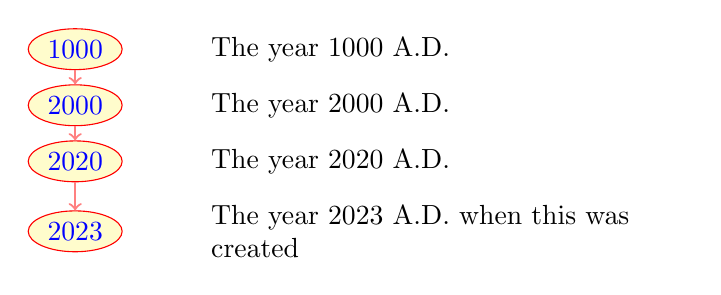
\begin{tikzpicture}[yscale=0.5,%
		   year/.style={draw=red,text=blue,fill=yellow!20,shape=ellipse,inner sep=2pt},
		   description/.style={rectangle,align=left,text width=60mm,anchor=west},
		   timeline/.style={->,thick,red!50}]

	    \foreach \year/\desc [count=\y] in {%
	       1000/The year 1000 A.D.,%
	       2000/The year 2000 A.D.,%
	       2020/The year 2020 A.D.,%
	       2023/The year 2023 A.D. when this was created%
	       } { \ifnum\y=1 \node[description](\y){\desc};
		   \else\node[description,below=1ex of \z](\y){\desc};
		   \fi
		   \node[year](y-\y) [left=of \y] {\year};
		   \ifnum\y>1\draw[timeline] (y-\z)-- (y-\y);\fi
		   \global\let\z=\y% for drawing from last node
	       }
	\end{tikzpicture}
	}
\end{frame}

\begin{frame}
	\frametitle{Timeline 2}
	\adjustbox{valign=c}{
	\newcounter{year2}
	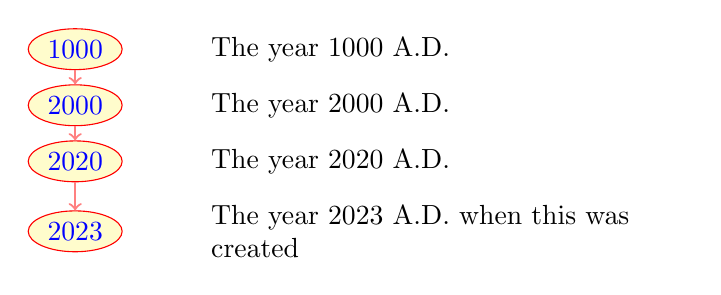
\begin{tikzpicture}[yscale=0.5,%
		   year/.style={draw=red,text=blue,fill=yellow!20,shape=ellipse,inner sep=2pt},
		   description/.style={rectangle,align=left,text width=60mm,anchor=west},
		   timeline/.style={->,thick,red!50}]

	    \foreach \year/\desc [count=\y] in {%
	       1000/The year 1000 A.D.,%
	       2000/The year 2000 A.D.,%
	       2020/The year 2020 A.D.,%
	       2023/The year 2023 A.D. when this was created%
	       } { \ifnum\y=1 \node[description](\y){\desc};
		   \else\node[description,below=1ex of \z](\y){\desc};
		   \fi
		   \node[year](y-\y) [left=of \y] {\year};
		   \ifnum\y>1\draw[timeline] (y-\z)-- (y-\y);\fi
		   \global\let\z=\y% for drawing from last node
	       }
	\end{tikzpicture}
	}
\end{frame}

\begin{frame}[fragile]
	\frametitle{Code snippets with Verb, verbatim, and minted}
	Notice that the \textbackslash begin\{frame\} of this frame is followed by [fragile], which is necessary for Verbatim to work properly\\\ \\
	Inline \textbackslash Verb example: \Verb#hello world#\\ \ \\
	Verbatim block example:
	\begin{verbatim}
block
hello
world
print('hello world')
	\end{verbatim}
	Better code snippets with Minted:
	\begin{minted}{python}
	def my_print(msg):
	    print(msg)
	\end{minted}
\end{frame}

\end{document}
